\section{Results: predicting GDP}

\begin{frame}{6.1 - Forecast exercise}
	\begin{itemize}
		\item sequential sample: start from 1993m7 - 2017m1, then increase sequentially by one month, for 36 months (3 years)
		\item for each sample: produce forecasts at 1, 2, 3 and 4 quarters aheead
		\item forecasts are produced for GDP and all features in $x_t$
		\item for each model, sample, horizon and features, compute RMSE = $\sqrt{(x_{t+h} - \hat{x}_{t+h})^2}$
		\item consider the average RMSE over the different samples
		\item RMSE are normalised to clear scale effects
		\item add a number of benchmarks to the 9 models for comparison
	\end{itemize}	
\end{frame}

\begin{frame}{6.2 - Results: GDP Nowcast}
	\begin{figure}[h]
		\centering
		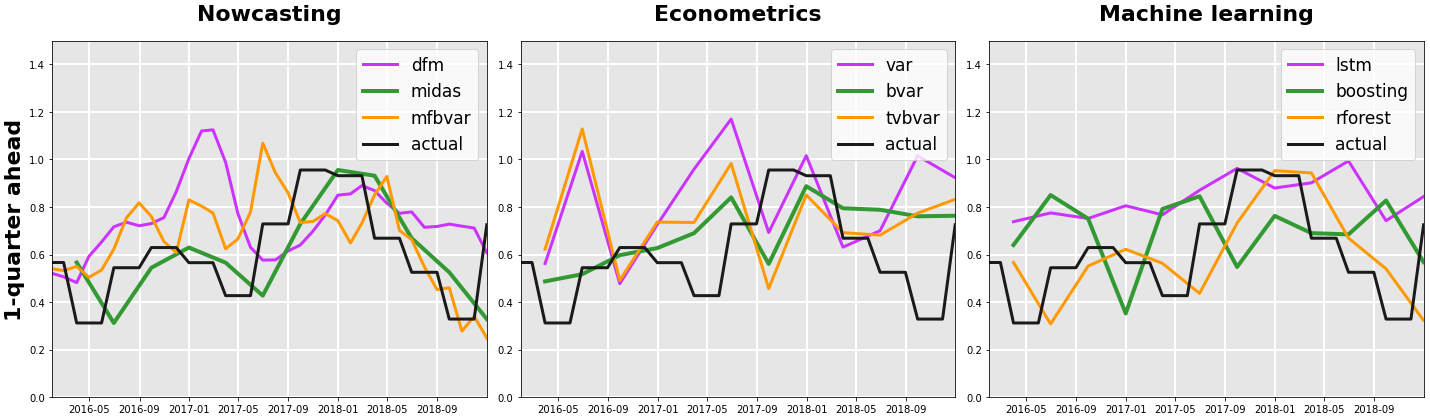
\includegraphics[width=1\linewidth]{im1}
		\caption{GDP nowcasts for the 9 models}
		\label{fig_62_1}
	\end{figure}
\end{frame}

\begin{frame}{6.2 - Results: GDP Nowcast}
\begin{figure}[h]
	\centering
	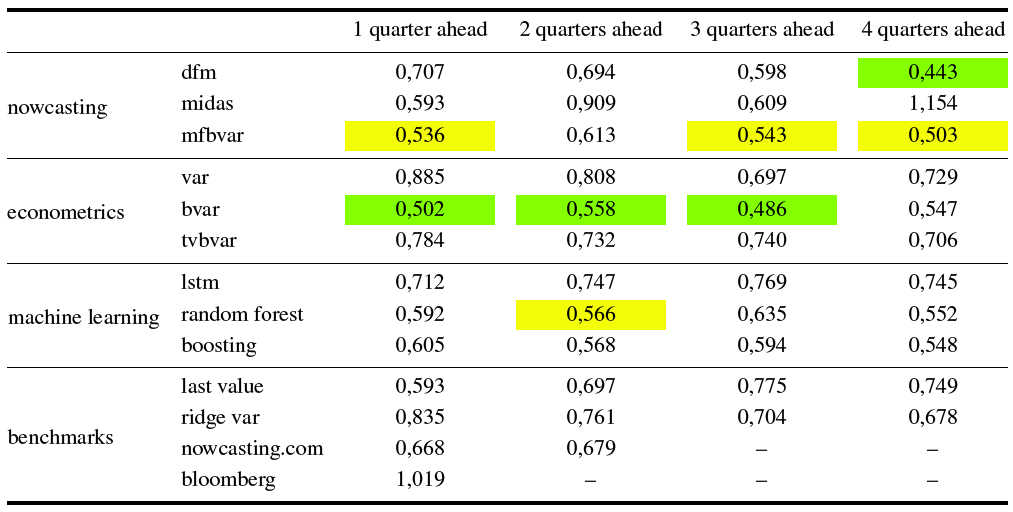
\includegraphics[width=.9\linewidth]{im2}
	\caption{RMSE on GDP predictions}
	\label{fig_62_2}
\end{figure}
\end{frame}

\begin{frame}{6.2 - Results: GDP Nowcast}
\begin{figure}[h]
	\centering
	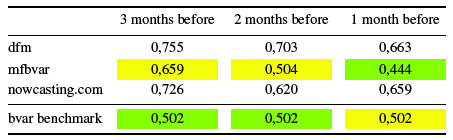
\includegraphics[width=.6\linewidth]{im3}
	\caption{RMSE on GDP nowcasts: 1, 2 and 3 months before release}
	\label{fig_62_3}
\end{figure}
\end{frame}

\begin{frame}{6.2 - Results: GDP Nowcast}
\begin{figure}[h]
	\centering
	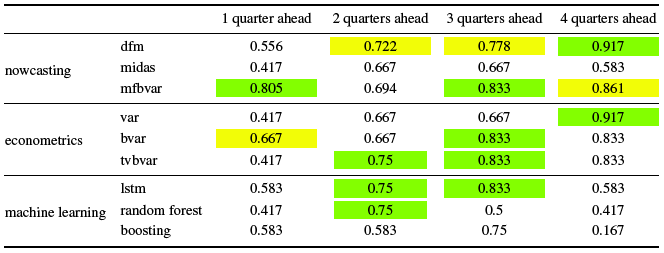
\includegraphics[width=.9\linewidth]{im4}
	\caption{Percentage of correct direction prediction}
	\label{fig_62_4}
\end{figure}
\end{frame}

\begin{frame}{6.3 - Conclusions: GDP Nowcast}
	\begin{itemize}
	\item BVAR and MF-BVAR dominate for both RMSE and direction
	\item BVAR best one quarter before release, MFBVAR best one month before
	\item not clear which one is best 2 months before release
	\item other good nowcasts models: MIDAS, random forest, naive last value predictor
	\item other models overfit
	\end{itemize}	
\end{frame}

